% !TEX root = ../Tesi_Triennale_PMNS.tex

\chapter[Segnali di GW da BNS]{Segnali di onde gravitazionali da BNS}
\label{chapter:segnaleGWdaBNS}
%    \begin{center}
%    	$\smallsim 3$ pagine
%    \end{center}
%    
%    Breve spiegazione su cos'è una neutron star.

Una stella di neutroni è la fase finale dell'evoluzione stellare in seguito alla cessazione delle reazioni di fusione nucleare degli elementi leggeri al suo interno
per stelle con massa tale che

\begin{equation}
   	\SI{10}{\solarmass} < M < \SI{25}{\solarmass}
   	\label{eqn:massNS}
\end{equation}
Accade dunque che, in una certa fase del collasso, le densità estremamente alte possono portare gli elettroni a interagire con i protoni, attraverso il fenomeno della cattura elettronica, portando alla formazione di neutroni (e neutrini). Date le densità estreme della stella di neutroni, rimane incertezza sulle equazioni di stato della materia.\cite{hobson2006general}

Una stella di neutroni (NS) è resa stabile, contro il collasso dovuto alla forza di gravità, non da pressioni termiche come per il sole, ma da forze legate al principio di esclusione di Pauli e interazioni nucleari tra i neutroni. Queste forze hanno effetti solo sopra le densità nucleari, che spiega perché le NS sono sono così compatte (una NS ha una massa poco superiore rispetto alla massa solare in un raggio di $\smallsim$10 km)\cite{hartle2003gravity}

%    ALTRO?

%    Sistemi binari di neutron star e perché emettono GW.

\begin{wrapfigure}{r}{0.5\textwidth}
	\vspace{-15pt}
	\begin{center}
		%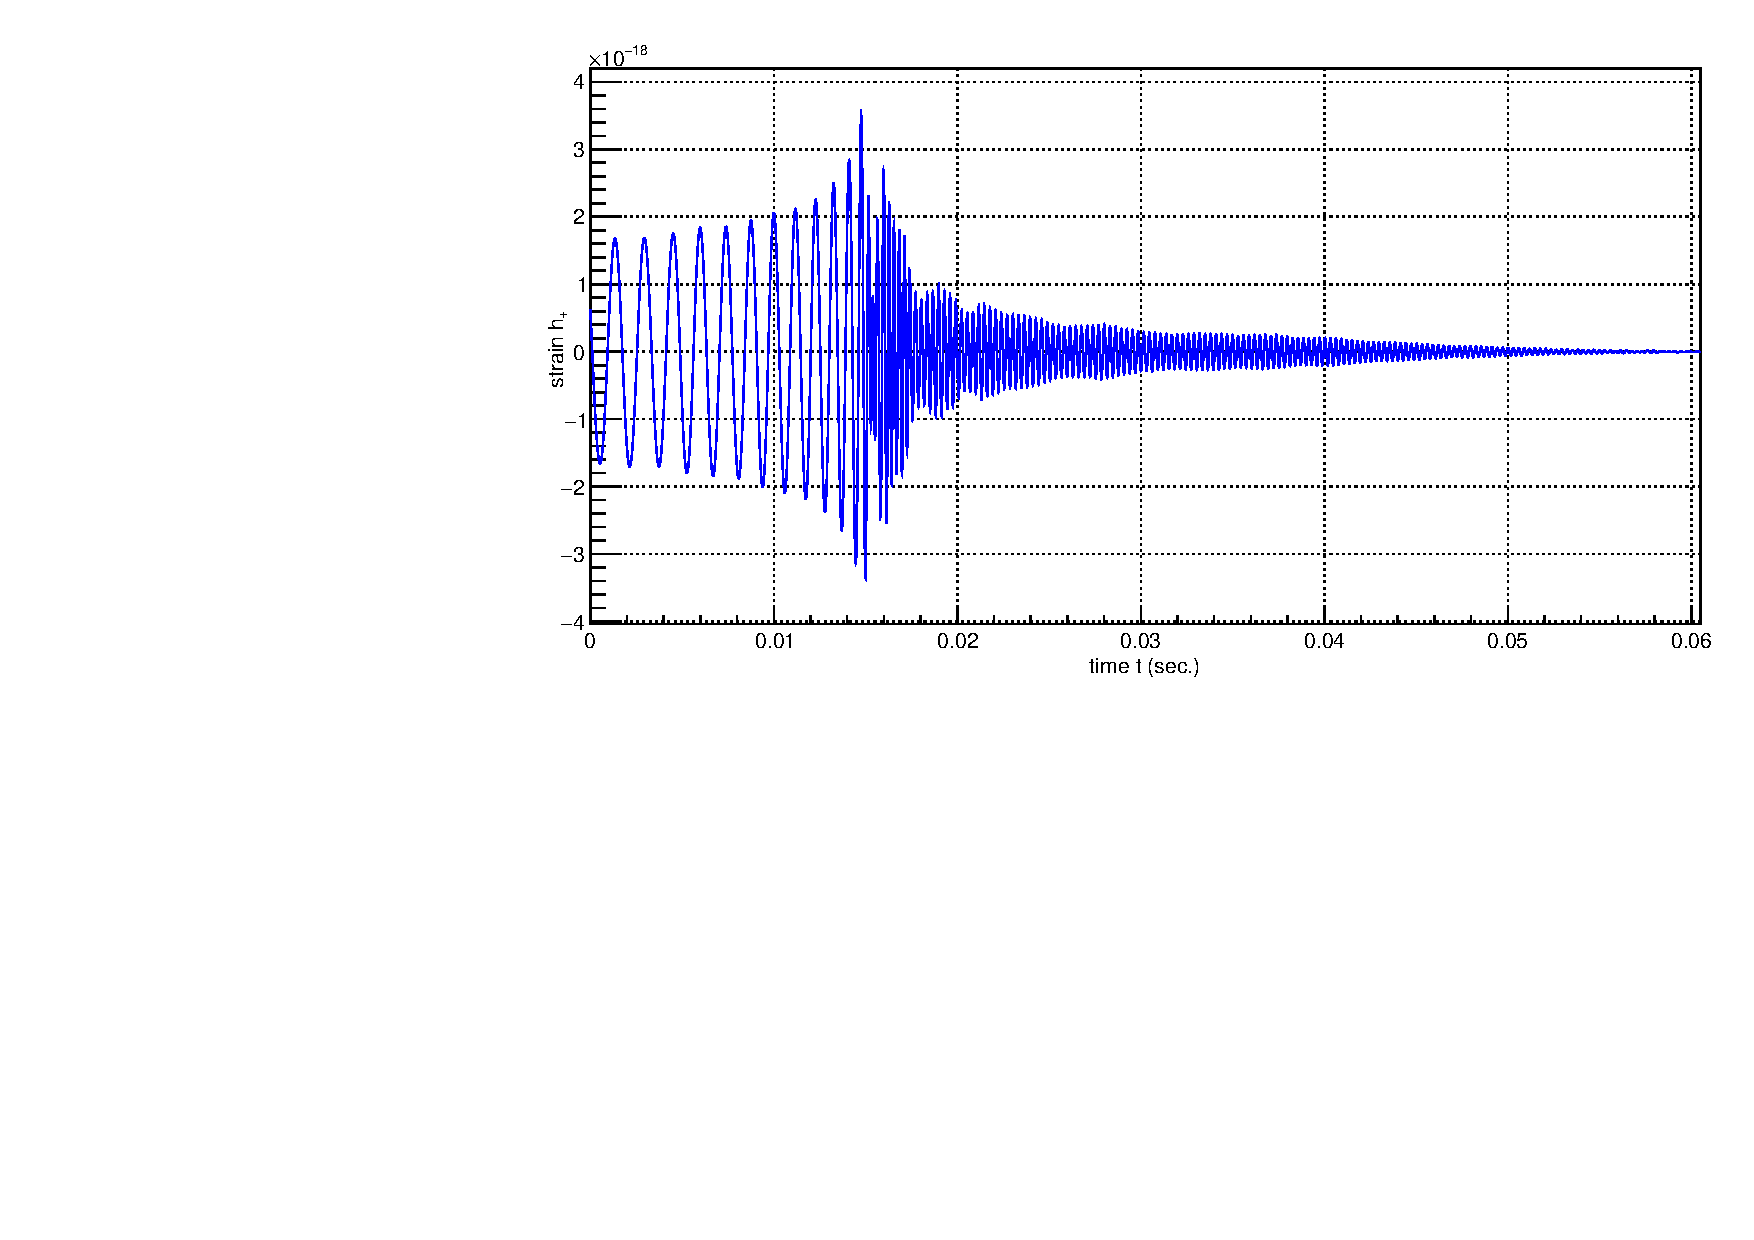
\includegraphics[width=0.48\textwidth]{figures/forma_onda_+_APR4_q09}
		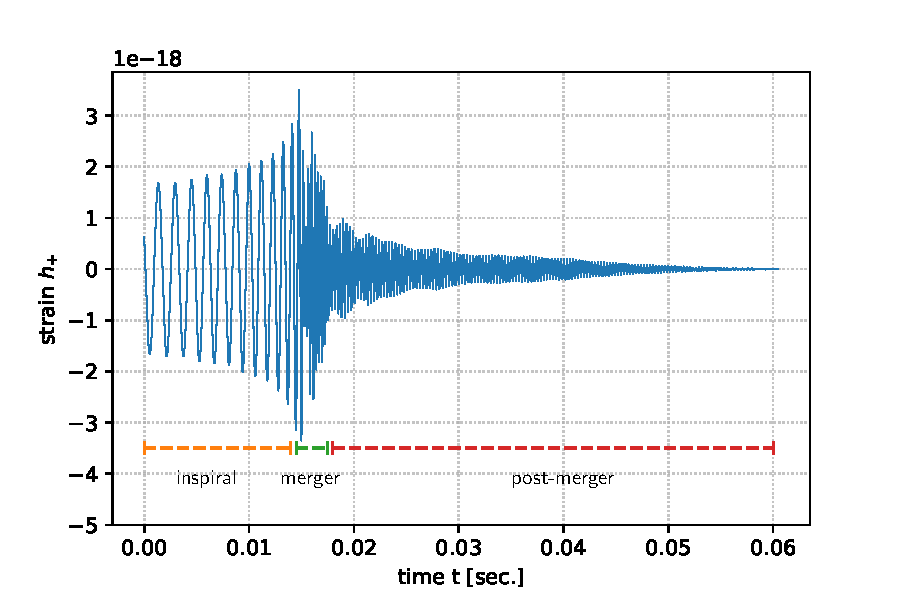
\includegraphics[width=0.55\textwidth]{figures/Capitolo_1/APR4.pdf}
	\end{center}
	\vspace{-10pt}
	\caption{Forma d'onda per la coalescenza di una BNS con equazione di stato APR4, con una divisione qualitativa tra le diverse fasi}
	\label{fig:forma_onda_APR4}
	\vspace{-10pt}
\end{wrapfigure}

Un sistema binario di stelle di neutroni (BNS), ovvero una coppia di NS che, legato attraverso la forza di attrazione gravitazionale, ruota attorno al centro di massa, emette segnali di onda gravitazionale (GW) che possono essere interpretati come fase di inspiral, merger e post-merger.

La lunga fase di spiraleggiamento consiste nelle due stelle che ruotano attorno al centro di massa e, a causa dell'emissione di energia sotto forma di onde gravitazionali, il raggio delle orbite diminuisce portando ad un incremento in ampiezza e frequenza della GW, producendo il caratteristico "chirp". Questa è l'unica fase che viene descritta con un approccio analitico.

La fase di spiraleggiamento termina con i due oggetti che si scontrano dando inizio alla fase di merger e quindi, dopo la fusione, al post-merger che in base alle proprietà iniziali del sistema può portare a forme d'onda e oggetti diversi.	Mentre la fase di merger dura pochi millisecondi, la fase di post-merger genera un segnale quasi-stazionario. Queste due fasi risultano più complesse da modellare, per cui si fa per il loro studio affidamento a metodi numerici. \cite{maggiore2008gravitational}

\section[Frequenze caratteristiche]{Frequenze caratteristiche di merger e post-merger}

Una BNS realistica presenta una massa compresa tra $\smallsim\SI{2.4}{\solarmass}$ e $\smallsim\SI{2.8}{\solarmass}$ e una differenza tra le due componenti che è di $\smallsim20\%$ o minore. 
A partire dal segnale di GW, in particolare nelle fasi di merger e post-merger, possono essere ottenute informazioni sull'equazione di stato della materia a densità nucleari e, da un'analisi spettrale, informazioni sulla tidal deformability (deformabilità mareale) delle due stelle.


\begin{wrapfigure}{r}{0.5\textwidth}
	\vspace{-15pt}
	\begin{center}
		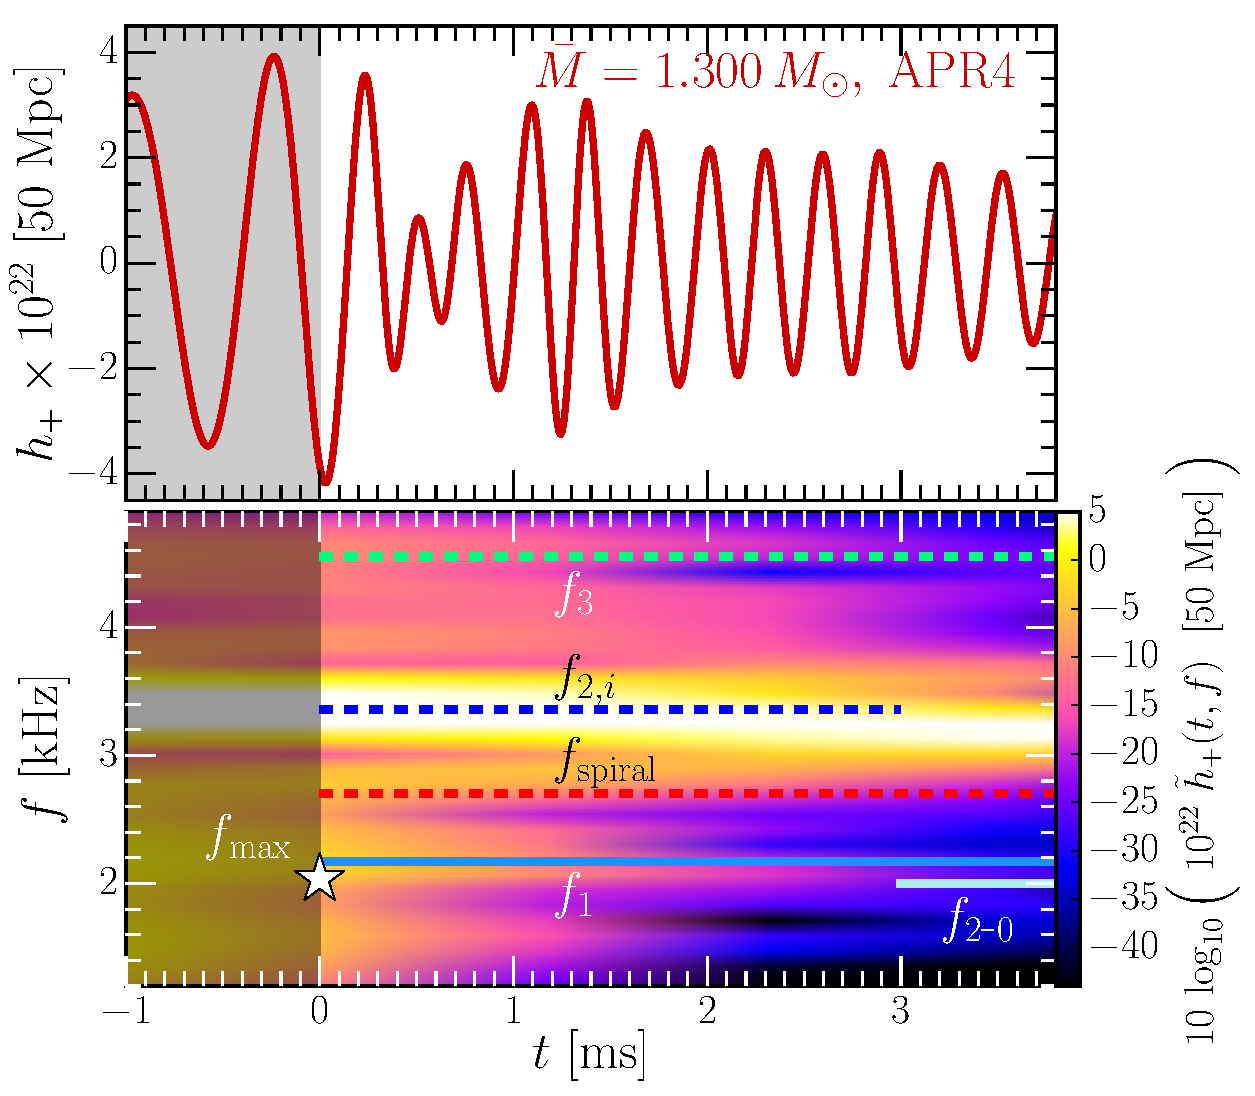
\includegraphics[width=0.5\textwidth]{figures/Capitolo_1/GW_spectrogram_short_APR4-q10-M1300.pdf}
	\end{center}
	\vspace{-10pt}
	\caption{Forma d'onda e relativo spettrogramma per il merger di una BNS con equazione di stato APR4 (morbida), presa da \cite{Rezzolla_2016}}
	\label{fig:spettrogramma_merger_APR4}
	\vspace{-25pt}
\end{wrapfigure}

Osservando dunque lo spettro del segnale di onda gravitazionale di merger, in particolare per binarie ccon masse che non differiscono per più del 20\%, questo presenterà alcune proprietà\cite{Rezzolla_2016}:
\begin{itemize}
   	\item la frequenza della GW al massimo di ampiezza $f_{max}$ è legata in modo quasi-universale con la tidal deformability delle due stelle;
   	\item le frequenze $f_1$, $f_{2,i}$ e $f_3$ rappresentano i picchi principali visibili dall'osservazione del post-merger, tra le quali si ottiene la seguente relazione empirica:
   	\begin{equation}
   		f_{2,i}\simeq\frac{f_1 + f_3}{2} 
   		\label{eqn:f1_2_3}
   	\end{equation} 
   	il picco $f_1$ è legato alla compattezza delle stelle, mentre il picco $f_{2,i}$ è legato al raggio della configurazione non rotante più massiva e corrisponde al modo fondamentale della NS ipermassiva con l=2=m;
\end{itemize}

\begin{itemize}
   	\item si identifica in alcuni casi un altro picco $f_{2-0}$ che si riferisce all'accoppiamento tra il modo fondamentale con l=2=m e il modo con simmetria assiale, cioè con l=2 e m=0;
   	\item il picco $f_{spiral}$ associato alla deformazione spiraleggiante dovuta alla rotazione, è però impossibile da misurare in calcoli numerici e si utilizzano dunque i valori prodotti da considerazioni analitiche. Si nota infine che $f_{spiral}$ coincide per molte EOS (in particolare EOS rigide) con la frequenza $f_1$, mentre per altre (EOS morbide) non si ha questa corrispondenza.
\end{itemize}

%	FORSE UN PO' CONFUSO

\begin{wrapfigure}{r}{0.5\textwidth}
	\vspace{-15pt}
	\begin{center}
		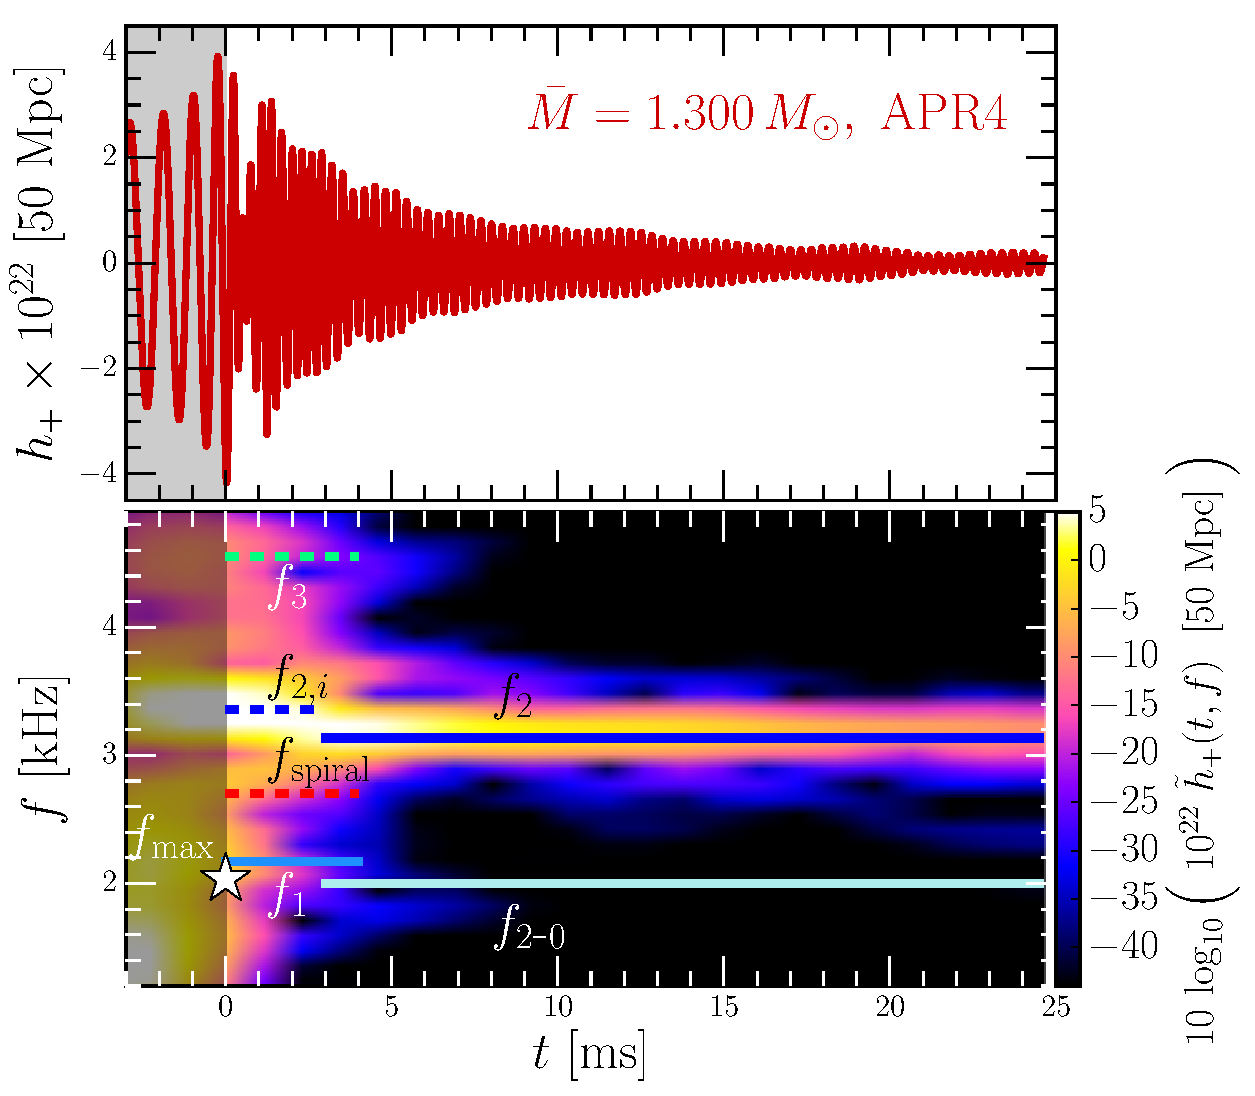
\includegraphics[width=0.5\textwidth]{figures/Capitolo_1/GW_spectrogram_APR4-q10-M1300.pdf}
	\end{center}
	\vspace{-10pt}
	\caption{Forma d'onda e relativo spettrogramma per il post-merger di una BNS con equazione di stato APR4, presa da \cite{Rezzolla_2016}}
	\label{fig:spettrogramma_postmerger_APR4}
	\vspace{-40pt}
\end{wrapfigure}

Nella fase di post-merger, nei casi in cui il sistema non collassa immediatamente in un buco nero, evidenziando nella forma d'onda una fase di ringdown in cui il segnale si spegne, l'unica frequenza a sopravvivere è il picco $f_2$, spariscono gli altri picchi, lasciando solo $f_{2-0}$ a basse energie.

È poi possibile trovare diverse relazioni quantitative che legano le frequenze osservate con le proprietà stellari, che risultano particolarmente utili come verifica delle previsioni teoriche.

%    Cenno sulle equazioni di stato.

%    Proprietà delle forme d'onda: merger e post-merger.

%    Brevissimi cenni sulle relazioni tra proprietà della forma d'onda e proprietà stellari.

%    \lipsum[1]\cite{sarin2020evolution}

%    \lipsum[2]\cite{Rezzolla_2016}.




\section{Oggetto residuo}
\label{section:residual}

Ci sono quattro possibili risultati della coalescenza di due stelle di neutroni, in base alle masse delle stelle e dalle loro equazioni di stato. 
Data la massa dell'oggetto residuo $M$, facendo riferimento alla figura \ref{fig:EvoluzioneBNS}:
\begin{itemize}
	\item $M\gtrsim 1.5 M_{TOV}$ \footnote{$M_{TOV}$ è detta massa di Tolman-Oppenheimer-Volkoff e indica la massa massima che può avere una stella di neutroni non rotante}: il sistema collassa immediatamente in un buco nero seguendo il percorso A\textrightarrow B\textrightarrow C;
	\item $1.2 M_{TOV} \lesssim M \lesssim 1.5 M_{TOV}$: l'oggetto rimanente è una stella di neutroni ipermassiva, che collassa in un buco nero in un tempo $\lesssim 1$s, seguendo A\textrightarrow B\textrightarrow D\textrightarrow E;		
	\item $M_{TOV} \lesssim M \lesssim 1.2 M_{TOV}$: rimane una stella di neutroni supermassiva che è destinata a collassare in un buco nero in un tempo di 10 \textdiv $10^4$s, secondo il percorso A\textrightarrow B\textrightarrow D\textrightarrow F\textrightarrow G;		\item $M\lesssim M_{TOV}$: rimane una stella di neutroni stabile, secondo il percorso A\textrightarrow B\textrightarrow D\textrightarrow F\textrightarrow H \cite{sarin2020evolution}.	
\end{itemize}
\begin{center}
	\begin{figure}[ht]
		\centering
		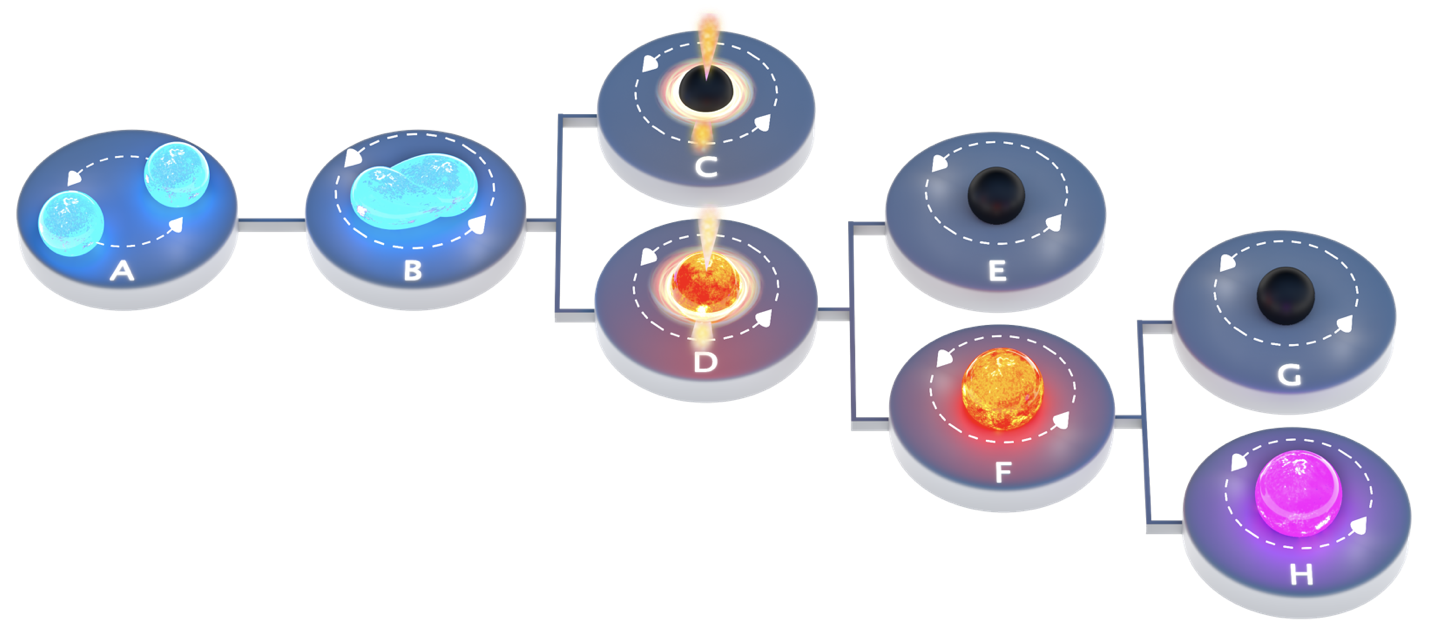
\includegraphics[scale=0.25, angle=0]{figures/Capitolo_1/MagnetarEvolution.png}
		\setlength{\belowcaptionskip}{-20pt}
		\caption{Rappresentazione pittorica del destino del residuo del merger di un sistema binario di stelle di neutroni, presa da \cite{sarin2020evolution}}
		\label{fig:EvoluzioneBNS}
	\end{figure}
\end{center}

Veloce descrizione delle possibili espulsioni di kilonovae

Descrizione mezza pagina dei $\gamma$ bursts

\subsection{Formazione diretta un black hole}	
\begin{wrapfigure}{r}{0.5\textwidth}
	\vspace{-30pt}
	\begin{center}
		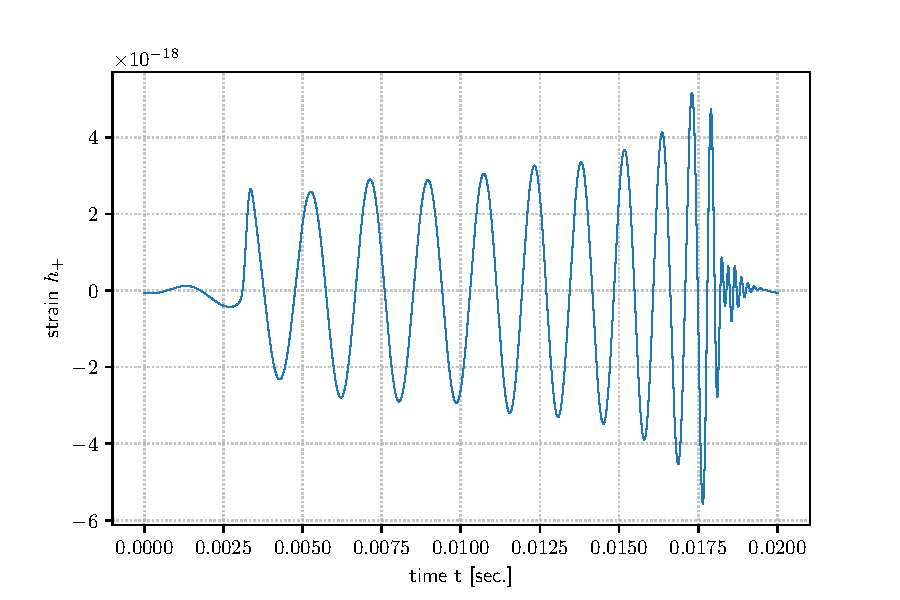
\includegraphics[width=0.5\textwidth]{figures/Capitolo_1/SHT2.2.pdf}
	\end{center}
	\vspace{-10pt}
	\caption{Forma d'onda per la coalescenza di una BNS con equazione di stato SHT2, in cui le masse sono tali da portare il sistema a collassare immediatamente in un BH, producendo nella fase di post merger il ringdown}
	\label{fig:FormaOndaBH}
	\vspace{-10pt}
\end{wrapfigure}

La formazione diretta di un buco nero dopo la coalescenza implica, come si osserva in figura \ref{fig:FormaOndaBH} lo spegnimento del segnale, con un collasso quasi sferico che genera delle onde gravitazionali minime\cite{sarin2020evolution}.

Questo tipo di segnale ha la particolarità, al contrario degli altri casi di post-merger, di ammattere uno studio analitico attraverso metodi perturbativi relativamente semplici (decrescita esponenziale con un tempo caratteristico legato alla massa del buco nero)\cite{maggiore2018gravitational}.

\subsection{Formazione di una NS ipermassiva}	

\begin{wrapfigure}{r}{0.5\textwidth}
	\vspace{-20pt}
	\begin{center}
		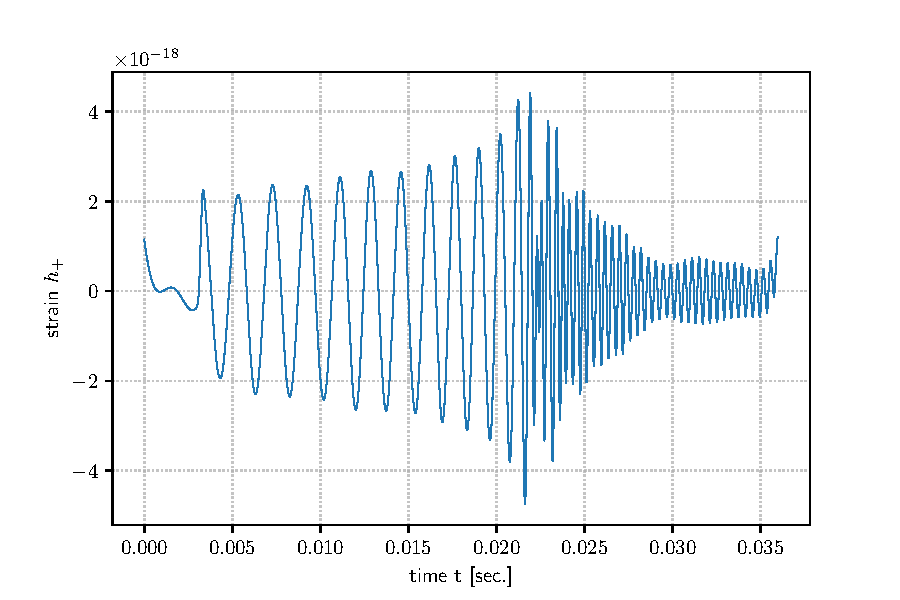
\includegraphics[width=0.5\textwidth]{figures/Capitolo_1/SHT2.0.pdf}
	\end{center}
	\vspace{-10pt}
	\caption{Forma d'onda per la coalescenza di una BNS con equazione di stato SHT2, in cui le masse sono tali da portare il sistema a formare una NS ipermassiva, producendo nella fase di post merger un segnale visibile}
	\label{fig:FormaOndaToNS}
	\vspace{-20pt}
\end{wrapfigure}

La maggior parte dei merger di stelle di neutroni porta alla formazione di stelle di neutroni ipermassive, supermassive o stabili. 

Una stella di neutroni ipermassiva è tale da avere una massa superiore al massimo in massa per una stella rotante uniformemente $M_{TOV}$, ma non collassa per la rotazione differenziale, cioè il fenomeno per cui le sue diverse parti ruotano con velocità angolare differente che permette una maggiore stabilità rispetto a stelle non rotanti o rotanti uniformemente \cite{Baumgarte_2000}, e per il supporto di gradienti termici. Nel momento in cui la stella rallenta la sua rotazione e/o si raffredda il supporto alla sua stessa massa termina e la stella collassa in un buco nero. 
Nel caso in cui la stella ipermassiva abbia massa tale che $M \gtrsim 1.2 M_{TOV}$ la rotazione uniforme non può dare sufficiente supporto centrifugo per evitare il collasso, per cui la stella collassa non appena la rotazione differenziale termina \cite{sarin2020evolution}.



pronto
	
pronto

pronto

pronto

pronto

pronto

pronto

pronto

pronto

\subsection{Formazione di una NS supermassiva}
\subsection{Formazione di una NS stabile}
Continuo descrizione possibili oggetti finali\cite{sarin2020evolution}
